\documentclass{article}
\usepackage[utf8]{inputenc} % 支持UTF-8编码
\usepackage{xeCJK} % 支持中文
\usepackage{graphicx} % 引入用于插入图片的宏包
\usepackage{hyperref} % 引入超链接宏包
\usepackage{amsmath}

\usepackage{geometry}
\geometry{
  a4paper,
  left=20mm,
  right=20mm,
  top=30mm,
  bottom=30mm
}

% 设置行距为1.5倍
\usepackage{setspace}
\linespread{1.75}

\begin{document}

\title{\textbf{
GFN1000 与自然对话\\
中英双语对照翻译版
}} % 文章标题
\date{}
\maketitle % 生成标题

\setcounter{secnumdepth}{0} % 禁止章节编号,但仍添加到目录
\tableofcontents
\newpage

\section{Text 2 from The Beginnings of Western Science/ \textit{David C. Lindberg}}
\begin{center}
CHAPTER THREE 第三章\\
ARISTOTLE'S PHILOSOPHY OF NATURE 亚里士多德的自然哲学\\
\end{center}
\textbf{Life and Works}\\
\noindent1\\
Aristotle (fig. 3.1) was born in 384 B.C. in the northern Greek town of Stagira, into a privileged family. His father was personal physician to the Macedonian king, Amyntas II (grandfather of Alexander the Great). Aristotle had the advantage of an exceptional education: at age seventeen, he was sent to Athens to study with Plato. He remained in Athens as a member of Plato’s Academy for twenty years, until Plato’s death about 347. Aristotle then spent several years in travel and study, crossing the Aegean Sea to Asia Minor and its coastal islands. During this period he undertook biological studies, and he encountered Theophrastus (from the island of Lesbos), who was to become his pupil and lifetime colleague. He returned to Macedonia in 342 to become the tutor of the young Alexander (later “the Great”). In 335, when Athens fell under Macedonian rule, Aristotle returned to the city and began to teach in the Lyceum, a public garden frequented by teachers. He remained there, establishing an informal school, until shortly before his death in 322.\\
亚里士多德(图 3.1)公元前 384 年出生于希腊北部的斯塔基拉镇,出生于一个特权家庭。他的父亲是马其顿国王阿敏塔斯二世(亚历山大大帝的祖父)的私人医生。亚里士多德拥有接受卓越教育的优势:17 岁时,他被送到雅典跟随柏拉图学习。他在雅典作为柏拉图学园的一员待了二十年,直到公元前 347 年柏拉图去世。之后,亚里士多德花了数年时间游历和学习,横渡爱琴海前往小亚细亚及其沿海岛屿。在此期间,他进行了生物学研究,并遇到了泰奥弗拉斯托斯(来自莱斯博斯岛),后者后来成为他的学生和终生同事。公元前 342 年,他回到马其顿,成为年轻的亚历山大(后来的 “大帝”)的导师。公元前 335 年,当雅典落入马其顿统治时,亚里士多德回到这座城市,开始在吕克昂讲学,吕克昂是一个教师常去的公共花园。他留在那里,建立了一所非正式的学校,直到公元前 322 年去世前不久。\\

\noindent2\\
In the course of his long career as student and teacher, Aristotle systematically and comprehensively addressed the major philosophical issues of his day. He is credited with more than 150 treatises, approximately 30 of which have come down to us. The surviving works appear to consist mainly of lecture notes or unfinished treatises not intended for wide circulation; whatever their exact origin, they were obviously directed to other philosophers, including advanced students. In modern translation, they occupy well over a foot of bookshelf, and they present a philosophical system overwhelming in power and scope. It is out of the question for us to survey the whole of Aristotle’s philosophy, and we must be content with examining the fundamentals of his philosophy of nature—beginning with his response to positions taken by the pre-Socratics and Plato.\\
在他作为学生和教师的漫长职业生涯中,亚里士多德系统而全面地探讨了他那个时代的主要哲学问题。他被认为著有超过 150 篇论文,其中约 30 篇流传至今。现存的作品似乎主要由讲稿或未完成的论文组成,这些作品并非为广泛流传而创作;无论其确切来源如何,它们显然是面向其他哲学家的,包括高年级学生。在现代译本中,它们占据了书架上一英尺多的空间,并且呈现了一个在影响力和范围上都令人惊叹的哲学体系。我们不可能全面审视亚里士多德的整个哲学体系,我们必须满足于研究他的自然哲学的基本原理 —— 从他对前苏格拉底哲学家和柏拉图所持观点的回应开始。\\

\noindent\textbf{Metaphysics and Epistemology 形而上学与认识论}\\
\noindent3\\
Through his long association with Plato, Aristotle had, of course, become thoroughly versed in Plato’s theory of forms. Plato had drastically diminished (without totally rejecting) the reality of the material world observed by the senses. Reality in its perfect fullness, Plato argued, is found only in the eternal forms, which are dependent on nothing else for their existence. The objects that make up the sensible world, by contrast, derive their characteristics and their very being from the forms; it follows that sensible objects exist only derivatively or dependently.\\
通过与柏拉图的长期交往,亚里士多德当然已经对柏拉图的形式理论了如指掌。柏拉图极大地贬低了(但并未完全否定)感官所观察到的物质世界的现实性。柏拉图认为,只有在永恒的形式中才能找到完美且完整的现实,这些形式的存在不依赖于其他任何东西。相比之下,构成可感知世界的物体,其特征和存在本身都源于形式;由此可见,可感知物体只是派生的或依赖性地存在。\\

\noindent4\\
Aristotle refused to accept this diminished, dependent status that Plato assigned to sensible objects. They must exist fully and independently, for in Aristotle’s view they were what make up the real world. Moreover, the traits that give an individual object its character do not, Aristotle argued, have a prior and separate existence in a world of forms, but belong to the object itself. There is no perfect form of a dog, for example, existing independently in the world of forms and replicated imperfectly in individual dogs, imparting to them their attributes. For Aristotle, there were just individual dogs. These dogs certainly shared a set of attributes—for otherwise we would not be entitled to call them “dogs”—but these attributes exist in, and belong to, individual dogs.\\
亚里士多德拒绝接受柏拉图赋予可感知对象的这种被贬低的、依赖的地位。它们必须完全且独立地存在,因为在亚里士多德看来,它们构成了现实世界。此外,亚里士多德认为,赋予单个对象特性的特质,并非在形式世界中先于对象且独立存在,而是属于对象本身。例如,不存在一种完美的狗的形式,独立存在于形式世界中,并在个体狗身上不完美地复制,赋予它们属性。对亚里士多德来说,只有个体的狗。这些狗当然共享一组属性 —— 否则我们就无权称它们为 “狗”—— 但这些属性存在于个体狗之中,且属于个体狗。\\

\noindent5\\
Perhaps this way of viewing the world has a familiar ring. Making individual sensible objects the primary realities (“substances,” Aristotle called them) will seem like good common sense to most readers of this book, and probably struck Aristotle’s contemporaries the same way. But if it makes good common sense, can it also be good philosophy? That is, can it deal successfully, or at least plausibly, with the difficult philosophical issues raised by the pre - Socratics and Plato—the nature of the fundamental reality, epistemological concerns, and the problem of change and stability? Let us take up these problems one by one.\\
也许这种看待世界的方式听起来很熟悉。将单个可感知对象视为首要的现实(亚里士多德称之为 “实体”),对这本书的大多数读者来说,似乎是很符合常识的,而且很可能亚里士多德同时代的人也有同样的看法。但如果这符合常识,那它也能成为好的哲学吗?也就是说,它能否成功地,或者至少看似合理地处理前苏格拉底哲学家和柏拉图提出的那些棘手的哲学问题 —— 即基本现实的本质、认识论问题以及变化与稳定的问题?让我们逐一探讨这些问题。\\

\noindent6\\
The decision to locate reality in sensible, corporeal objects does not yet tell us very much about reality—only that we should look for it in the sensible world. Already in Aristotle’s day, any philosopher would demand to know more: one thing he would demand to know was whether the corporeal materials of daily experience (wood, water, air, stone, metal, flesh, etc.) are themselves the fundamental, irreducible constituents of things, or whether they are composites of still more fundamental stuff. Aristotle addressed this question by drawing a distinction between properties and their subjects. He maintained (as most of us would) that a property has to be the property of something; we call that something its “subject.” To be a property is to belong to a subject; properties cannot exist independently.\\
将现实定位在可感知的有形物体上这一决定,并没有告诉我们太多关于现实的信息 —— 只是表明我们应该在可感知的世界中去寻找现实。在亚里士多德的时代,任何哲学家都会要求了解更多:其中一个他们想要知道的事情是,日常经验中的有形物质(木材、水、空气、石头、金属、肉体等)本身是否就是事物的基本、不可再分的组成部分,或者它们是否是由更基本的物质构成的复合物。亚里士多德通过区分属性及其主体来解决这个问题。他坚持(就像我们大多数人会认为的那样),属性必须是某物的属性;我们把那个某物称为它的 “主体”。作为一种属性就是要属于一个主体;属性不能独立存在。\\

\noindent7\\
Individual corporeal objects, then, have both properties (color, weight, texture, and the like) and something other than properties to serve as their subject. These two roles are played by “form” and “matter,” respectively. Corporeal objects are “composites” of form and matter—form consisting of the properties that make the thing what it is, matter serving as the subject or substratum for the form. A white rock, for example, is white, hard, heavy, and so forth, by virtue of its form; but matter must also be present, to serve as subject for the form, and this matter brings no properties of its own to its union with form. (Aristotle’s doctrine will be further discussed in chap. 12, below, in connection with medieval attempts to clarify and extend it.)\\
那么,单个有形物体既有属性(颜色、重量、质地之类),也有属性之外的某种东西作为其主体。这两种角色分别由 “形式” 和 “质料” 来扮演。有形物体是形式和质料的 “复合物”—— 形式由使事物成为其自身的属性构成,质料则作为形式的主体或基质。例如,一块白色的石头,凭借其形式而是白色的、坚硬的、沉重的等等;但质料也必须存在,以作为形式的主体,并且这种质料在与形式结合时不会带来其自身的任何属性。(亚里士多德的这一学说将在下面的第 12 章中,结合中世纪为澄清和扩展它所做的尝试,作进一步讨论。)\\

\noindent8\\
We can never, in actuality, separate form and matter; they are presented to us only as a unitary composite. If they were separable, we should be able to put the properties (no longer the properties of anything) in one pile, the matter (absolutely propertyless) in another—an obvious impossibility. But if form and matter can never be separated, is it not meaningless to speak of them as the real constituents of things? Isn’t this a purely logical distinction, existing in our minds, but not in the external world? Surely not for Aristotle, and perhaps not for us; most of us would think twice before denying the real existence of cold or red, although we can never collect a bucket of either one. In short, Aristotle once again surprises us by using commonsense notions to build a persuasive philosophical edifice.\\
实际上,我们永远无法将形式和质料分离;它们只以一个统一的复合物的形式呈现给我们。如果它们是可分离的,我们就应该能够把属性(不再是任何事物的属性)放在一堆,把质料(完全没有属性)放在另一堆 —— 这显然是不可能的。但是,如果形式和质料永远无法分离,那么把它们说成是事物真正的组成部分,岂不是没有意义?这难道不是一种纯粹的逻辑区分,只存在于我们的头脑中,而不存在于外部世界吗?对于亚里士多德来说肯定不是,或许对我们来说也不是;我们大多数人在否认冷或红的真实存在之前都会三思,尽管我们永远无法收集到一桶冷或一桶红。简而言之,亚里士多德再次用常识性的概念构建了一座有说服力的哲学大厦,这让我们感到惊讶。\\

\noindent9(重点理解认识过程)\\
Aristotle’s claim that the primary realities are concrete individuals surely has epistemological implications, since true knowledge must be knowledge of truly real things. By this criterion, Plato’s attention was naturally directed toward the eternal forms, knowable through reason or philosophical reflection. Aristotle’s metaphysics of concrete individuals, by contrast, directed his quest for knowledge toward the material world of individuals, of nature, and of change—a world encountered through the senses.\\
亚里士多德主张首要的现实是具体的个体,这无疑具有认识论上的意义,因为真正的知识必定是关于真正真实事物的知识。按照这个标准,柏拉图的注意力自然指向了永恒的形式,这些形式可通过理性或哲学反思来认识。相比之下,亚里士多德关于具体个体的形而上学,将他对知识的追求引向了个体、自然和变化的物质世界 —— 一个通过感官所接触到的世界。\\

\noindent10\\
Aristotle’s epistemology is complex and sophisticated. It must suffice here to indicate that the process of acquiring knowledge begins with sense experience. From repeated sense experience follows memory; and from memory, by a process of “intuition” or insight, the experienced investigator is able to discern the universal features of things. By the repeated observation of dogs, for example, an experienced dog breeder comes to know what a dog really is; that is, he comes to understand the form or definition of a dog, the crucial traits without which an animal cannot be a dog. Note that Aristotle, no less than Plato, was determined to grasp the universal traits or properties of things; but, unlike his teacher, Aristotle argued that one must start with the individual material thing. Once we grasp the universal properties or definition, we can put it to use as the premise of deductive demonstrations.\\
亚里士多德的认识论既复杂又精妙。在此只需指出,获取知识的过程始于感官经验。从反复的感官经验中产生记忆;而从记忆出发,通过 “直觉” 或洞察的过程,经验丰富的研究者能够辨别事物的普遍特征。例如,通过对狗的反复观察,一位经验丰富的养狗人会逐渐了解狗的真正本质;也就是说,他会逐渐理解狗的形式或定义,即那些没有它们动物就不能成为狗的关键特征。请注意,亚里士多德和柏拉图一样,都决心把握事物的普遍特征或属性;但与他的老师不同的是,亚里士多德认为必须从单个物质事物开始。一旦我们掌握了普遍属性或定义,我们就可以将其用作演绎论证的前提。\\

\noindent11\\
Knowledge is thus gained by a process that begins with experience (a term broad enough, in some contexts, to include common opinion or the reports of distant observers). In that sense knowledge is empirical; nothing can be known apart from such experience. But what we learn by this “inductive” process does not acquire the status of true knowledge until put into deductive form; the end - product is a deductive demonstration (nicely illustrated in a Euclidean proof) beginning from universal definitions as premises. Although Aristotle discussed both the inductive and deductive phases (the latter far more than the former) in the acquisition of knowledge, he stopped considerably short of later methodologists, especially in the analysis of induction.\\
因此,知识是通过一个从经验开始的过程获得的(在某些语境中,“经验” 这个词足够宽泛,包括普遍观点或遥远观察者的报告)。从这个意义上说,知识是经验性的;没有这样的经验,就无法知晓任何事物。但是,我们通过这种 “归纳” 过程所学到的东西,在被纳入演绎形式之前,并不具有真正知识的地位;最终的成果是一个从普遍定义作为前提出发的演绎论证(在欧几里得证明中得到了很好的例证)。尽管亚里士多德在知识获取过程中讨论了归纳和演绎两个阶段(对后者的讨论远多于前者),但与后来的方法论学者相比,他的探讨仍有很大差距,尤其是在对归纳的分析方面。\\

\noindent12\\
This is the theory of knowledge outlined by Aristotle in the abstract. Is it also the method actually employed in Aristotle’s own scientific investigations? Probably not—with perhaps an occasional exception. Like modern scientists, Aristotle did not proceed by following a methodological recipe book, but rather by rough and ready methods, familiar procedures that had proved themselves in practice. Somebody has defined science as “doing your damnedest, no holds barred”; when it came (for example) to his extensive biological researches, this is exactly what Aristotle did. It is not a surprise, and certainly no character defect, that Aristotle should, in the course of thinking about the nature and the foundations of knowledge, formulate a theoretical scheme (an epistemology) not perfectly consistent with his own scientific practice.\\
这就是亚里士多德概括性地勾勒出的知识理论。这也是他在自己的科学研究中实际采用的方法吗?很可能不是 —— 或许偶尔有例外。和现代科学家一样,亚里士多德并不是按照一本方法论的 “食谱” 来开展研究的,而是采用一些简便可行的方法,那些在实践中已被证明有效的常见程序。有人将科学定义为 “竭尽全力,毫无保留”;例如,当涉及到他广泛的生物学研究时,亚里士多德正是这样做的。亚里士多德在思考知识的本质和基础的过程中,制定出一个与他自己的科学实践并非完全一致的理论框架(一种认识论),这并不奇怪,当然也不是他的性格缺陷。\\

\noindent\textbf{Life and Works 生活和工作}\\
\noindent13\\
The problem of change had become a celebrated philosophical issue (within the quite small community of philosophers) in the fifth century B.C. In the fourth century, Plato had dealt with it by restricting change to the imperfect material replica of the changeless world of forms. For Aristotle, a distinguished naturalist who was philosophically committed to the full reality of the changeable individuals that make up the sensible world, the problem of change was a most pressing one.\\
在公元前 5 世纪,变化问题在(规模相当小的哲学家群体中)已成为一个著名的哲学议题。在公元前 4 世纪,柏拉图通过将变化限制在不变的形式世界的不完美物质复制品中来处理这个问题。对于亚里士多德这位在哲学上认定构成可感知世界的可变个体具有充分现实性的杰出博物学家来说,变化问题是一个最为紧迫的问题。\\

\noindent14\\
Aristotle’s starting point was the commonsense assumption that change is genuine. But this does not, by itself, get us very far; it remains to be demonstrated that the idea of change can withstand philosophical scrutiny; it must also be shown how change can be explained. Aristotle had various weapons in his arsenal by which to achieve these ends. The first was his doctrine of form and matter. If every object is constituted of form and matter, then Aristotle could make room for both change and stability by arguing that when an object undergoes change, its form changes (by a process of replacement, the new form replacing the old one) while its matter remains unchanged. Aristotle went on to argue that change in form takes place between a pair of opposites or contraries, one of which is the form to be achieved, the other its privation or absence. When the dry becomes wet, or the cold becomes hot, this is change from privation (dry or cold) to the intended form (wet or hot). Change, for Aristotle, is thus never random, but confined to the narrow corridor connecting pairs of contrary qualities; order is thus discernible even in the midst of change.\\
亚里士多德的出发点是一种常识性假设,即变化是真实存在的。但这本身并不能让我们走得太远;仍需证明变化的观念能够经受住哲学的审视;还必须说明如何解释变化。亚里士多德有各种 “武器” 来实现这些目标。第一个是他的形式与质料学说。如果每个物体都是由形式和质料构成的,那么亚里士多德可以通过论证当一个物体发生变化时,其形式发生变化(通过一种替换过程,新形式取代旧形式)而质料保持不变,从而为变化和稳定都留出空间。亚里士多德接着论证说,形式的变化发生在一对对立面或相反物之间,其中一个是要实现的形式,另一个是它的缺失或匮乏。当干的变湿,或冷的变热时,这就是从匮乏状态(干或冷)向预期形式(湿或热)的变化。因此,对亚里士多德来说,变化绝非随机的,而是局限于连接相反性质对的狭窄 “通道” 内;即使在变化之中,秩序也是可辨的。\\

\noindent15\\
A determined Parmenidean might protest that to this point the analysis does nothing to escape Parmenides’ objection to all change on the ground that inevitably it calls for the emergence of something out of nothing. Aristotle’s reply is found in his doctrine of potentiality and actuality. Aristotle would undoubtedly have granted that if the only two possibilities are being and non - being—that is, if things either exist or do not exist—then the transition from non - hot to hot would indeed involve passage from non - being to being (the nonexistence of hot to the existence of hot) and would thus be vulnerable to Parmenides’ objection. But Aristotle believed that the objection could be successfully circumvented by supposing that there are three categories associated with being instead of two: not just being and non - being, but (1) non - being, (2) potential being, and (3) actual being. If such is the state of things, then change can occur between potential being and actual being without non - being ever entering the picture. What Aristotle has in mind is perhaps most easily illustrated by examples from the biological realm. An acorn is potentially, but not actually, an oak tree. In becoming an oak tree, it becomes actually what it originally was only potentially. The change thus involves passage from potentiality to actuality—not from non - being to being, but from one kind or degree of being to another. Or for a pair of non - biological examples, a heavy body held above the earth falls in order to fulfill its potential of being situated with other heavy things about the center of the universe. And a sculptor, with mallet and hammer, reveals in actuality a shape that existed potentially within the original block of marble.\\
一个坚定的巴门尼德主义者可能会抗议说,到目前为止,这种分析并没有摆脱巴门尼德对所有变化的反对意见,因为变化不可避免地需要无中生有。亚里士多德的回答体现在他的潜能与现实学说中。亚里士多德无疑会承认,如果只有两种可能性,即存在和不存在 —— 也就是说,如果事物要么存在,要么不存在 —— 那么从非热到热的转变确实会涉及从不存在到存在的过渡(从热的不存在到热的存在),因此会受到巴门尼德反对意见的质疑。但亚里士多德认为,通过假设与 “存在” 相关的有三类而非两类,就可以成功地避开这一反对意见:不只是存在和不存在,而是(1)不存在,(2)潜在的存在,以及(3)现实的存在。如果情况是这样的话,那么变化就可以在潜在的存在和现实的存在之间发生,而不存在从不介入。亚里士多德的想法或许可以通过生物领域的例子最容易地加以说明。一颗橡子潜在地(而非现实地)是一棵橡树。在变成橡树的过程中,它成为了原本只是潜在的东西的现实形态。因此,这种变化涉及从潜能到现实的过渡 —— 不是从不存在到存在,而是从一种存在或存在程度到另一种存在或存在程度。或者举两个非生物的例子,一个被举在地球上方的重物下落,是为了实现它与宇宙中心附近的其他重物处于同一位置的潜能。而一位雕塑家用槌子和锤子,将原本潜在地存在于大理石原块中的形状变为现实。\\

\noindent16\\
If these arguments allow us to escape the logical dilemmas associated with the idea of change, and therefore to believe in its possibility, they do not yet tell us anything about the cause of change. Why should an acorn move from the status of potential oak tree to that of actual oak tree, or an object change from black to white, rather than remaining in its original state? Aristotle answered with an intricate, subtle, and not always consistent, theory of nature and causation. Given these difficulties, we will spare ourselves the pain of an exhaustive account and treat ourselves to the short version.\\
如果这些论证使我们能够摆脱与变化观念相关的逻辑困境,从而相信变化的可能性,那么它们尚未告诉我们任何有关变化原因的信息。为什么一颗橡子会从潜在的橡树状态转变为现实的橡树状态,或者一个物体为什么会从黑色变为白色,而不是保持其原始状态呢?亚里士多德用一个复杂、微妙且并非总是一致的自然与因果理论来回答。鉴于这些困难,我们将省去详尽阐述的麻烦,采用简短的版本。\\

\noindent17\\
The world we inhabit is an orderly one, in which things generally behave in predictable ways, Aristotle argued, because every natural object has a “nature”—an attribute (associated primarily with form) that makes the object behave in its customary fashion, provided no insurmountable obstacle intervenes—or, as a modern commentator has put it, “that within a thing which determines basically what that thing does when it is being itself.” For Aristotle, a brilliant zoologist, the growth and development of biological organisms were easily explained by the activity of such an inner driving force. An acorn becomes an oak tree because its nature is to do so. But the theory was applicable beyond biological growth and, indeed, beyond the biological realm altogether. Dogs bark, rocks fall, and marble yields to the hammer and chisel of the sculptor because of their respective natures. Ultimately, Aristotle argued, all change and motion in the universe can be traced back to the natures of things. For the natural philosopher, who by definition is interested in change and things capable of undergoing change, these natures are the central object of study.\\
亚里士多德认为,我们所居住的世界是一个有序的世界,在这个世界中,事物通常以可预测的方式运行,因为每个自然物体都有一种 “本性”—— 一种属性(主要与形式相关),这种属性使物体以其惯常的方式运行,前提是没有不可逾越的障碍介入 —— 或者,正如一位现代评论家所说,“事物内部的某种东西,它从根本上决定了事物在展现自身时的行为”。对于身为杰出动物学家的亚里士多德来说,生物有机体的生长和发育很容易通过这样一种内在驱动力的活动来解释。一颗橡子长成一棵橡树,是因为它的本性使然。但这一理论的适用范围超出了生物生长,实际上,完全超出了生物领域。狗吠、石头下落、大理石在雕塑家的锤子和凿子下成型,都是因为它们各自的本性。亚里士多德认为,归根结底,宇宙中的所有变化和运动都可以追溯到事物的本性。对于自然哲学家来说,根据定义,他们对变化以及能够发生变化的事物感兴趣,这些本性就是研究的核心对象。\\

\noindent18\\
To this general statement of Aristotle’s theory of “nature,” we need to add a qualification—namely, that an artificially produced object is a special case, for such an object possesses no nature other than the natures of its ingredients. If a chariot is constructed of wood and iron, the nature of wood and nature of iron do not yield to a composite “nature of a chariot.” By contrast, in the organic world the natures of the organs and tissues that make up an organism yield to the nature of the organism as a whole. The nature of the human body is not the sum of the natures of its various tissues and organs, but a unique nature characteristic of that living human as an organic whole.\\
对于亚里士多德 “本性” 理论的这一一般性陈述,我们需要补充一个限定条件 —— 即人工制造的物体是一个特殊情况,因为这样的物体除了其组成成分的本性之外,并不拥有其他本性。如果一辆战车是由木头和铁制成的,木头的本性和铁的本性并不会产生出一个复合的 “战车的本性”。相比之下,在有机世界中,构成生物体的器官和组织的本性服从于生物体作为一个整体的本性。人体的本性不是其各种组织和器官本性的总和,而是作为一个有机整体的活人所具有的独特本性。\\

\noindent19\\
With this theory of nature in mind, we can understand a feature of Aristotle’s scientific practice that has puzzled and distressed modern commentators and critics—namely, the absence from his work of anything resembling controlled experimentation. Unfortunately, such criticism overlooks Aristotle’s aims, which drastically limited his methodological options. If, as Aristotle believed, the nature of a thing is to be discovered through the behavior of that thing in its natural, unfettered state, then artificial constraints will merely interfere and corrupt. If, despite interference, the object behaves in its customary fashion, we have troubled ourselves for no purpose. If we set up conditions that prevent the nature of an object from revealing itself, all we have learned is that it can be interfered with to the point of remaining concealed. Contrived experimentation violates, rather than reveals, the natures of things. Aristotle’s scientific practice is not to be explained, therefore, as a result of stupidity or deficiency on his part—failure to perceive an obvious procedural improvement—but as a method compatible with the world as he perceived it and suited to the questions that interested him. Experimental science emerged not when, at long last, the human race produced somebody clever enough to perceive that artificial conditions would assist in the exploration of nature, but when a rich variety of conditions were fulfilled—including the emergence of questions to which such a procedure promised to provide answers.\\
牢记这一关于 “本性” 的理论,我们就能理解亚里士多德科学实践中的一个令现代评论家和批评家感到困惑和苦恼的特点 —— 即在他的著作中没有任何类似于控制实验的内容。不幸的是,这种批评忽视了亚里士多德的目标,这些目标极大地限制了他的方法论选择。如果像亚里士多德所认为的那样,事物的本性要通过该事物在其自然、不受束缚状态下的行为来发现,那么人为的限制只会产生干扰和破坏。如果尽管受到干扰,物体仍以其惯常的方式运行,那我们就是在无端自扰。如果我们设置的条件阻止了物体的本性显现,那我们所了解到的只是它可以被干扰到一直隐藏起来的程度。人为设计的实验不是揭示而是违背了事物的本性。因此,亚里士多德的科学实践不应被解释为他本人愚蠢或有缺陷的结果 —— 没能察觉到明显的程序改进 —— 而应被视为一种与他所认知的世界相符、适合他所感兴趣问题的方法。实验科学的出现,并不是因为人类最终产生了足够聪明的人,能够认识到人为条件将有助于探索自然,而是因为满足了各种各样的条件 —— 包括出现了这种程序有望提供答案的问题。\\

\noindent20\\
To complete our analysis of Aristotle’s theory of change, we must briefly consider the celebrated four Aristotelian causes. To understand a change or the production of an artifact is to know its causes (perhaps best translated “explanatory conditions and factors”). There are four of these: the form of a thing; the matter underlying that form, which persists through the change; the agency that brings about the change; and the purpose served by the change. These are called, respectively, formal cause, material cause, efficient cause, and final cause. To take an extremely simple example—the production of a statue—the formal cause is the shape given the marble, the material cause is the marble that receives this shape, the efficient cause is the sculptor, and the final cause is the purpose for which the statue is produced (perhaps the beautification of Athens or the celebration of one of its heroes). There are cases in which identifying one or another of the causes is difficult, or in which one or more causes merge, but Aristotle was convinced that his four causes provided an analytical scheme of general applicability.\\
为了完成对亚里士多德变化理论的分析,我们必须简要考虑著名的亚里士多德四因说。理解一种变化或一件人工制品的产生,就是要知晓其原因(或许最好翻译为 “解释性条件和因素”)。原因有四种:事物的形式;构成该形式基础且在变化中持续存在的质料;引发变化的主体;以及变化所服务的目的。它们分别被称为形式因、质料因、动力因和目的因。举一个极其简单的例子 —— 雕像的制作 —— 形式因是赋予大理石的形状,质料因是接受这种形状的大理石,动力因是雕塑家,目的因是制作雕像的目的(或许是为了美化雅典或纪念其一位英雄)。在有些情况下,识别其中某一个原因可能很困难,或者一个或多个原因会融合在一起,但亚里士多德坚信他的四因说提供了一个具有普遍适用性的分析框架。\\

\noindent21\\
We have said enough about the form - matter distinction to make clear what was meant by “formal” and “material” causes, and “efficient” cause is close enough to modern notions of causation to require no further comment; but “final” cause requires explanation. In the first place, the expression “final cause” is an English cognate derived from the Latin word finis, meaning “goal,” “purpose,” or “end,” and it has nothing to do with the fact that it often appears last in the list of Aristotelian causes. Aristotle argued, quite rightly, that many things cannot be understood without knowledge of purpose or function. To explain the arrangement of teeth in the mouth, for example, we must understand their functions (sharp teeth in front for tearing, molars in back for grinding). Or to take an example from the inorganic realm, it is not possible to grasp why a saw is made as it is without knowing the function the saw is meant to serve. Aristotle went so far as to give final cause priority over material cause, noting that the purpose of the saw determines the material (iron) of which it must be made, whereas the fact that we possess a piece of iron does nothing to determine that we will make it into a saw.\\
关于形式 - 质料的区分我们已经说得够多,足以阐明 “形式因” 和 “质料因” 的含义,并且 “动力因” 与现代的因果观念足够接近,无需进一步评论;但 “目的因” 需要解释。首先,“目的因”(final cause)这个表达是一个英语同源词,源自拉丁语单词 finis,意思是 “目标”“目的” 或 “终点”,它与它在亚里士多德的原因列表中常常排在最后这一事实并无关联。亚里士多德很正确地论证说,许多事物如果不了解其目的或功能就无法被理解。例如,要解释口腔中牙齿的排列,我们必须了解它们的功能(前面的尖牙用于撕裂,后面的臼齿用于研磨)。或者从无机领域举个例子,如果不知道锯子预期的功能,就不可能理解为什么锯子是这样制作的。亚里士多德甚至认为目的因优先于质料因,他指出锯子的目的决定了制作它所必须使用的材料(铁),而我们拥有一块铁这一事实并不能决定我们会把它做成锯子。\\

\noindent22\\
Perhaps the most important point to be made about final cause is its clear illustration of the role of purpose (the more technical term is “teleology”) in Aristotle’s universe. The world of Aristotle is not the inert, mechanistic world of the atomists, in which the individual atom pursues its own course mindless of all others. Aristotle’s world is not a world of chance and coincidence, but an orderly, organized world, a world of purpose, in which things develop toward ends determined by their natures. It would be unfair and pointless to judge Aristotle’s success by the degree to which he anticipated modern science (as though his goal was to answer our questions, rather than his own); it is nonetheless worth noting that the emphasis on functional explanation to which Aristotle’s teleology leads would prove to be of profound significance for all of the sciences and remains to this day a dominant mode of explanation within the biological sciences.\\
或许关于目的因最重要的一点是,它清晰地阐明了目的(更专业的术语是 “目的论”)在亚里士多德宇宙中的作用。亚里士多德的世界不是原子论者所认为的那种惰性的、机械的世界,在原子论者的世界里,单个原子盲目地沿着自己的轨迹运行,对其他原子毫不理会。亚里士多德的世界不是一个充满偶然和巧合的世界,而是一个有序、有组织的世界,一个有目的的世界,在这个世界里,事物朝着由它们的本性所决定的目标发展。以亚里士多德对现代科学的预见程度来评判他的成就,既不公平也毫无意义(就好像他的目标是回答我们的问题,而不是他自己的问题一样);尽管如此,值得注意的是,亚里士多德的目的论所导致的对功能解释的强调,将被证明对所有科学都具有深远的意义,并且直到今天,它仍然是生物科学中一种占主导地位的解释模式。\\

\noindent\textbf{Cosmology}\\
\noindent23\\
Aristotle not only devised methods and principles by which to investigate and understand the world: form and matter, nature, potentiality and actuality, and the four causes. In the process, he also developed detailed and influential theories regarding an enormous range of natural phenomena, from the heavens above to the earth and its inhabitants below.\\
亚里士多德不仅设计了用于研究和理解世界的方法和原则:形式与质料、本性、潜能与现实以及四因说。在此过程中,他还针对从天上到地下及其居民等极为广泛的自然现象,发展出了详尽且具有影响力的理论。\\

\noindent24\\
Let us start with the question of origins. Aristotle adamantly denied the possibility of a beginning, insisting that the universe must be eternal. The alternative—that the universe came into being at some point in time—he regarded as unthinkable, violating (among other things) Parmenidean strictures about something coming from nothing. Aristotle’s position on this question would prove troublesome for medieval Christian Aristotelians.\\
让我们从起源问题开始。亚里士多德坚决否认宇宙有开端的可能性,坚持认为宇宙必定是永恒的。另一种观点,即宇宙在某个时间点形成,他认为是不可想象的,因为这(除其他方面外)违反了巴门尼德关于无中生有的戒律。亚里士多德在这个问题上的立场将给中世纪的基督教亚里士多德主义者带来麻烦。\\

\noindent25\\
Aristotle considered this eternal universe to be a great sphere, divided into an upper and a lower region by the spherical shell in which the moon is situated. Above the moon is the celestial region; below is the terrestrial region; the moon, spatially intermediate, is also of intermediate nature. The terrestrial or sublunar region is characterized by birth, death, and transient change of all kinds; the celestial or supralunar region, by contrast, is a region of eternally unchanging cycles. That this scheme had its origin in observation would seem clear enough; in his On the Heavens, Aristotle noted that “in the whole range of time past, so far as our inherited records reach, no change appears to have taken place either in the whole scheme of the outermost heaven or in any of its proper parts.” If in the heavens we observe eternally unvarying circular motion, he continued, we can infer that the heavens are not made of the terrestrial elements, the nature of which (observation reveals) is to rise or fall in transient rectilinear motions. The heavens must consist of an incorruptible fifth element (there are four terrestrial elements): the quintessence (literally, the fifth essence) or aether. The celestial region is completely filled with this quintessence (no void space) and divided, as we shall see, into concentric spherical shells bearing the planets. It had, for Aristotle, a superior, quasi - divine status.\\
亚里士多德认为这个永恒的宇宙是一个巨大的球体,被月球所在的球壳分为上下两个区域。月球之上是天界,之下是地界;月球在空间上处于中间位置,其性质也具有中间性。地界或月下区域的特点是有生有死以及各种短暂的变化;相比之下,天界或月上区域则是一个永恒不变的循环区域。这种体系源于观察这一点似乎相当清楚;亚里士多德在他的《论天》中指出:“在过去的整个时间范围内,就我们继承的记录所及,最外层天体的整个结构或其任何固有部分似乎都没有发生过变化。” 他接着说,如果我们在天界观察到永恒不变的圆周运动,我们就可以推断出天界不是由地界元素构成的,因为(观察表明)地界元素的本性是在短暂的直线运动中上升或下降。天界必定由一种不可腐朽的第五元素(地界有四种元素)构成:即 “以太”(字面意思是第五种本质)。天界完全充满了这种以太(没有虚空),并且正如我们将看到的,被划分为承载行星的同心球壳。对亚里士多德来说,天界具有一种优越的、近乎神圣的地位。\\

\begin{figure} % [h]表示尽量让图片在此处显示,也可根据需要改为[t](顶部)、[b](底部)等
    \centering
    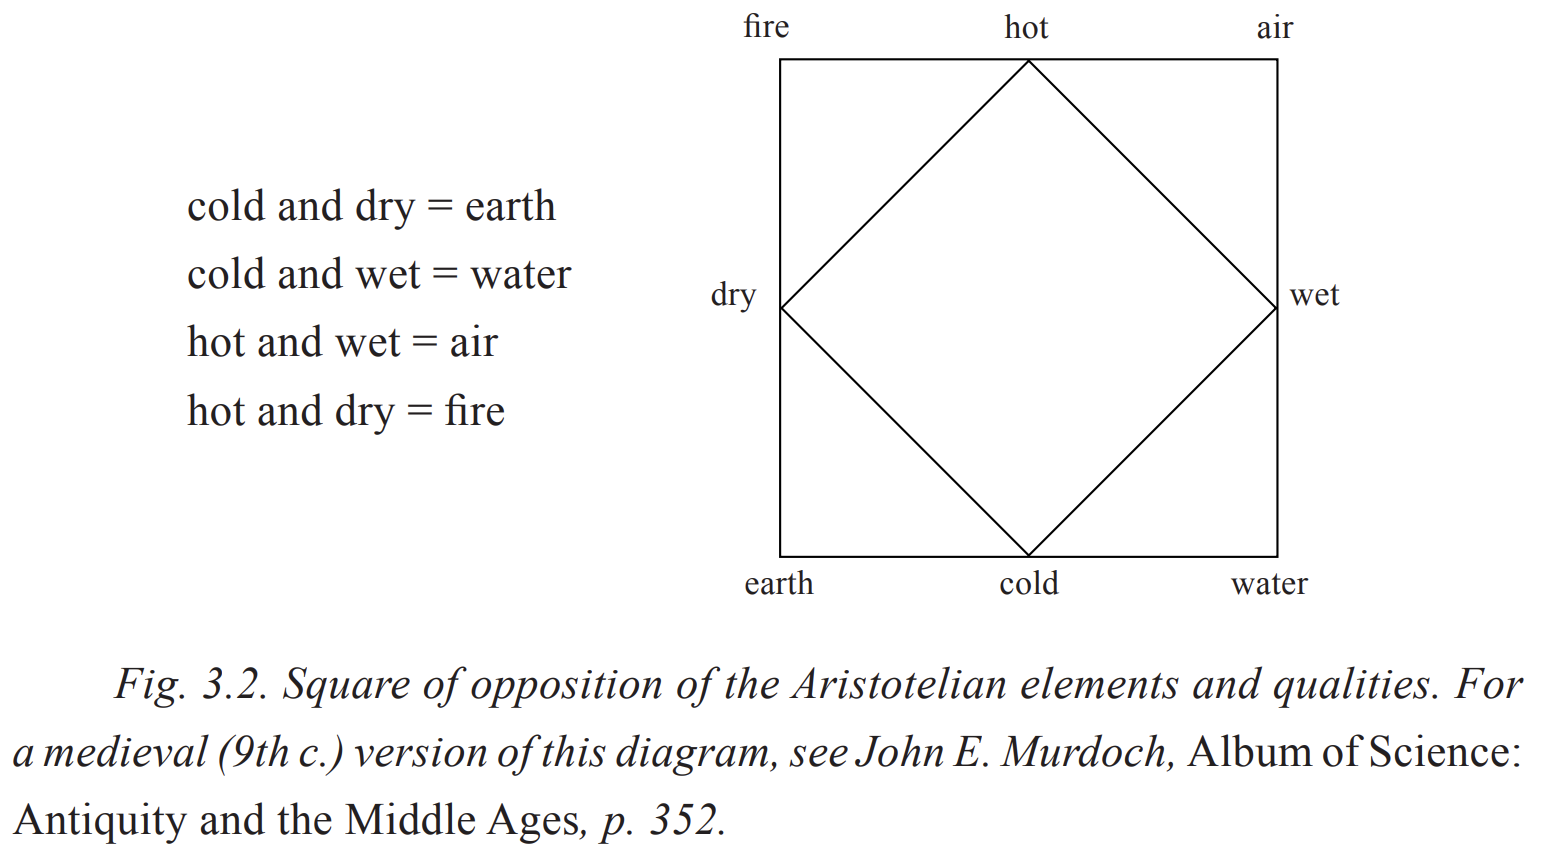
\includegraphics[width=0.75\linewidth]{image/Text2/Fig2.1.png} % 假设图片文件名为fig3.2.jpg,且与.tex文件在同一目录下,如果不在同一目录,需写完整路径

\end{figure}

\noindent26\\
The sublunar region is the scene of generation, corruption, and impermanence. Aristotle, like his predecessors, inquired into the basic element or elements to which the multitude of substances found in the terrestrial region can be reduced. He accepted the four elements originally proposed by Empedocles and subsequently adopted by Plato—earth, water, air, and fire. He agreed with Plato that these elements are in fact reducible to something even more fundamental; but he did not share Plato’s mathematical inclination and therefore refused to accept Plato’s regular solids and their constituent triangles. Instead, he expressed his own commitment to the reality of the world of sense experience by choosing sensible qualities as the ultimate building blocks. Two pairs of qualities are crucial: hot - cold and wet - dry. These combine in four pairs, each of which yields one of the elements (see fig. 3.2). Notice the use made once again of contraries. There is nothing to forbid any of the four qualities being replaced by its contrary, as the result of outside influence. If water is heated, so that the cold of water yields to hot, the water is transformed into air. Such a process easily explains changes of state (from solid to liquid to vapor, and conversely), but also more general transmutation of one substance into another. On such a theory as this, alchemists could easily build.\\
月下区域是生成、腐朽和无常的场所。亚里士多德和他的前辈们一样,探究了地界中众多物质可归结为的一种或几种基本元素。他接受了恩培多克勒最初提出、随后被柏拉图采用的四种元素——土、水、气和火。他同意柏拉图的观点,即这些元素实际上可以归结为更基本的东西;但他没有柏拉图那样的数学倾向,因此拒绝接受柏拉图的正多面体及其构成三角形。相反,他通过选择可感知的性质作为最终的构成要素,表达了自己对感官经验世界真实性的坚持。两对性质至关重要:热 - 冷和湿 - 干。它们以四对的形式组合,每一对产生一种元素(见图3.2)。注意这里再次使用了相反的性质。由于外界影响,没有什么能阻止这四种性质中的任何一种被其相反的性质所取代。如果水被加热,使得水的冷让位于热,水就会变成气。这样一个过程很容易解释状态的变化(从固体到液体再到气体,反之亦然),也能解释一种物质更普遍地转变为另一种物质。炼金术士很容易在这样一种理论基础上进行研究。\\

\noindent27\\
The various substances that make up the cosmos totally fill it, leaving no empty space. To appreciate Aristotle’s view, we must lay aside our almost automatic inclination to think atomistically; we must conceive material things not as aggregates of tiny particles but as continuous wholes. If it is obvious that, say, a loaf of bread is composed of crumbs separated by small spaces, there is no reason not to suppose that those spaces are filled by some finer substance, such as air or water. And there is certainly no simple way of demonstrating, nor indeed any obvious reason for believing, that water and air are anything but continuous. Similar reasoning, applied to the whole of the universe, led Aristotle to the conclusion that the universe is full, a plenum, containing no void space. This claim would be attacked by medieval scholars.\\
构成宇宙的各种物质完全充满了宇宙,没有留下任何空隙。为了理解亚里士多德的观点,我们必须抛开几乎是本能的原子论思维倾向;我们必须把物质事物设想为连续的整体,而不是微小粒子的集合。比如说,一块面包显然是由被小空隙隔开的面包屑组成的,那么没有理由不假定这些空隙被某种更精细的物质,比如空气或水所填满。而且肯定没有简单的方法来证明,实际上也没有任何明显的理由让人相信,水和空气不是连续的。将类似的推理应用于整个宇宙,亚里士多德得出结论,宇宙是充满的,是一个 “充实” 的状态,不存在虚空。这一主张将受到中世纪学者的抨击。\\

\noindent28\\
Aristotle defended this conclusion with a variety of arguments, such as the following. The speed of a falling body is dependent on the density of the medium through which it falls—the less the density, the swifter the motion of the falling body. It follows that in a void space (density zero), there is nothing to slow the descent of the body, from which we would be forced to conclude that the body would fall with infinite speed—a nonsensical notion, since it implies that the body could be at two places at the same time. Critics have frequently noted that this argument can just as well be taken to prove that the absence of resistance does not entail infinite speed as to prove that void does not exist. The point is, of course, well taken. However, we need to understand that Aristotle’s denial of the void did not rest on this single piece of reasoning. In fact, this was but one small part of a lengthy campaign against the atomists, in which Aristotle battled the notion of void space (or void place) with a variety of arguments, some more and some less persuasive.\\
亚里士多德用多种论据来捍卫这一结论,如下所述。一个落体的速度取决于它下落所通过的介质的密度——密度越小,落体的运动就越快。由此可知,在虚空(密度为零)中,没有任何东西能减缓物体的下落,据此我们将不得不得出物体将以无限速度下落的结论——这是一个荒谬的概念,因为这意味着物体可以同时处于两个位置。批评者经常指出,这个论据既可以用来证明没有阻力并不意味着速度无限,也可以用来证明虚空不存在。当然,这一点说得很有道理。然而,我们需要明白,亚里士多德对虚空的否定并不基于这单一的推理。事实上,这只是他反对原子论者的漫长论战中的一小部分,在这场论战中,亚里士多德用各种论据来反驳虚空(或虚空位置)的概念,这些论据有的更有说服力,有的则不那么有说服力。 \\

\noindent29\\
In addition to being hot or cold and wet or dry, each of the elements is also heavy or light. Earth and water are heavy, but earth is the heavier of the two. Air and fire are light, fire being the lighter of the two. In assigning levity to two of the elements, Aristotle did not mean (as we might, if we were making the claim) simply that they are less heavy, but that they are light in an absolute sense; levity is not a weaker version of gravity, but its contrary. Because earth and water are heavy, it is their nature to descend toward the center of the universe; because air and fire are light, it is their nature to ascend toward the periphery (that is, the periphery of the terrestrial region, the spherical shell that contains the moon). If there were no hindrances, therefore, earth and water would collect at the center; because of its greater heaviness, earth would achieve a lower position, forming a sphere at the very center of the universe; water would collect in a concentric spherical shell just outside it. Air and fire naturally ascended, but fire, owing to its greater levity, occupies the outermost region, with air as a concentric sphere just inside it. In the ideal case (in which there are no mixed bodies and nothing prevents the natures of the four elements from fulfilling themselves), the elements would thus form a set of concentric spheres: fire on the outside, followed by air and water, and finally earth at the center (see fig. 3.3). But in reality, the world is composed largely of mixed bodies, one always interfering with another, and the ideal is never attained. Nonetheless, the ideal arrangement defines the natural place of each of the elements; the natural place of earth is at the center of the universe, of fire just inside the sphere of the moon, and so forth.\\
除了热或冷、湿或干之外,每种元素还具有重或轻的属性。土和水是重的,而土是两者中较重的。气和火是轻的,火是两者中较轻的。亚里士多德赋予其中两种元素 “轻性”,他的意思并不是(如果我们提出这样的主张的话可能会认为的那样)仅仅指它们没那么重,而是指它们在绝对意义上是轻的;轻性不是重力的较弱形式,而是它的对立面。因为土和水是重的,它们的本性是向宇宙中心下降;因为气和火是轻的,它们的本性是向周边上升(也就是地界的周边,即包含月球的球壳)。因此,如果没有阻碍,土和水会聚集在中心;由于土更重,它会处于更低的位置,在宇宙的正中心形成一个球体;水会聚集在紧挨着它的一个同心球壳中。气和火自然上升,但由于火更轻,它占据最外层区域,气则作为紧挨着它的一个同心球。在理想情况下(没有混合物体,且没有任何东西阻止四种元素的本性得以实现),这些元素会形成一组同心球:火在最外层,接着是气和水,最后土在中心(见图 3.3)。但在现实中,世界主要由混合物体组成,它们总是相互干扰,理想状态从未达到。尽管如此,这种理想排列定义了每种元素的 “自然位置”;土的自然位置在宇宙中心,火的自然位置在月球球壳内侧,等等。\\

\begin{figure}
    \centering
    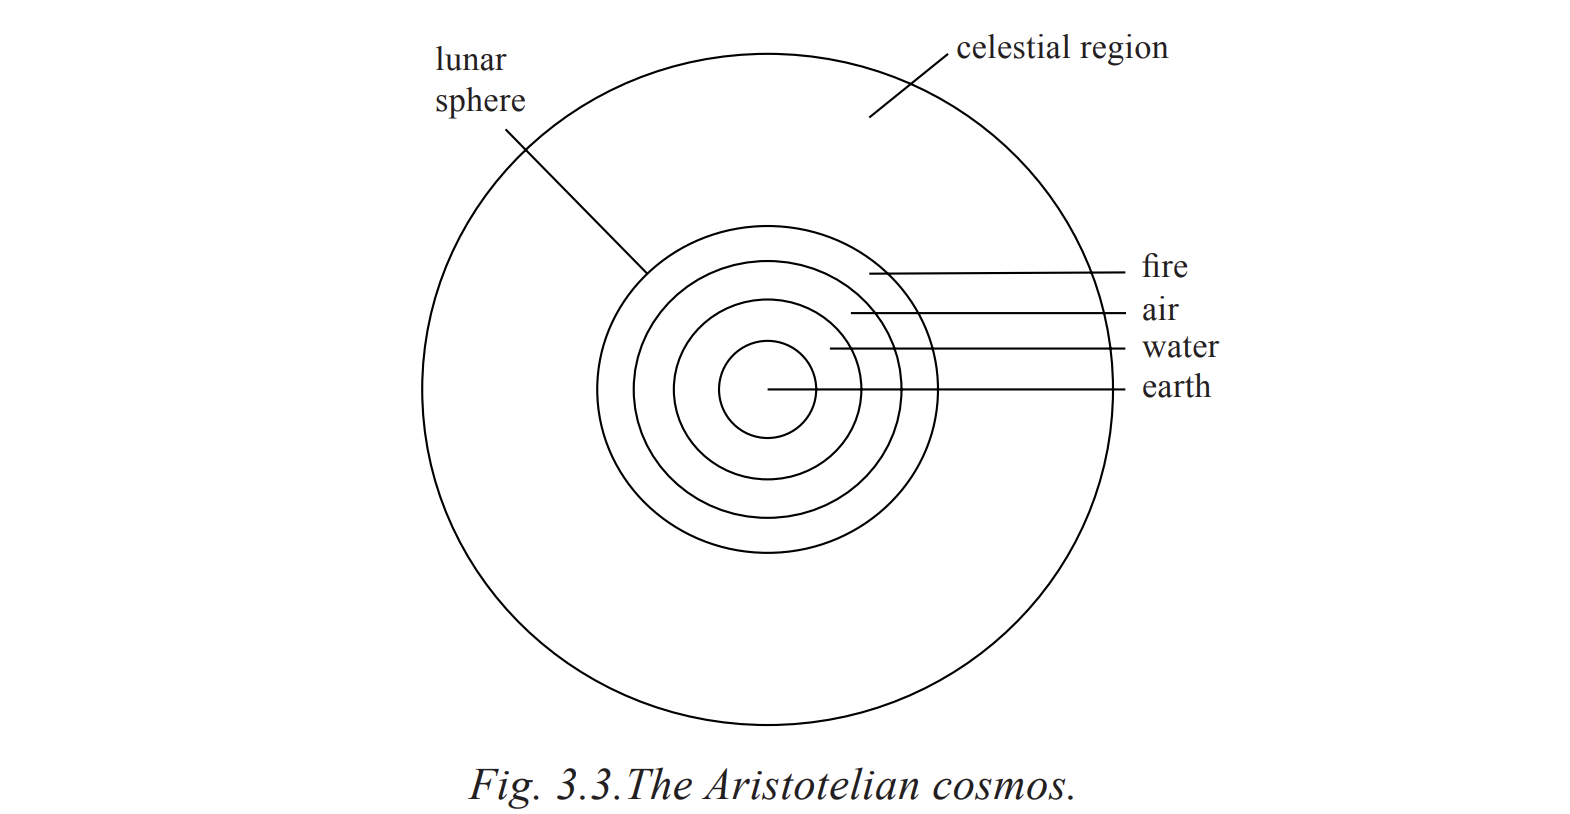
\includegraphics[width=0.75\linewidth]{image/Text2/Fig2.2.png}
\end{figure}

\noindent30\\
It must be emphasized that the arrangement of the elements is spherical. Earth collects at the center to form the earth, and it too is spherical. Aristotle defended this belief with a variety of arguments. Arguing from his natural philosophy, he pointed out that since the natural tendency of earth is to move toward the center of the universe, it must arrange itself symmetrically about that point. But he also called attention to observational evidence, including the circular shadow cast by the earth during a lunar eclipse and the fact that north - south motion by an observer on the surface of the earth alters the apparent position of the stars. Aristotle even reported an estimate by mathematicians of the earth’s circumference (400,000 stades = about 45,000 miles, roughly 1.8 times the modern value). The sphericity of the earth, thus defended by Aristotle, would never be forgotten or seriously questioned. The widespread myth that medieval people believed in a flat earth is of modern origin.\\
必须强调的是,元素的排列是球形的。土聚集在中心形成地球,地球本身也是球形的。亚里士多德用各种论据来捍卫这一观点。从他的自然哲学角度进行论证,他指出,由于土的自然倾向是向宇宙中心移动,它必定会围绕该点对称排列。但他也提请人们注意观测证据,包括月食时地球投射的圆形阴影,以及地球上的观察者进行南北移动时会改变星星的视位置这一事实。亚里士多德甚至提到了数学家对地球周长的估计(400,000斯塔德 = 约45,000英里,大约是现代数值的1.8倍)。亚里士多德如此捍卫的地球球形说,从未被遗忘或受到严重质疑。中世纪人认为地球是平的这一广泛流传的说法是现代才有的误解。 \\

\noindent31\\
Finally, we must note one of the implications of this cosmology, namely that space, instead of being a neutral, homogeneous backdrop (analogous to our modern notion of geometrical space) against which events occur, has properties. Or to express the point more precisely, ours is a world of space, whereas Aristotle’s was a world of place. Heavy bodies move toward their place at the center of the universe not because of a tendency to unite with other heavy bodies located there, but simply because it is their nature to seek that central place; if by some miracle the center happened to be vacant (a physical impossibility in an Aristotelian universe, but an interesting imaginary state of affairs), it would remain the destination of every heavy body.\\
最后,我们必须注意到这种宇宙论的一个含义,即空间并非是事件发生的中性、同质的背景(类似于我们现代的几何空间概念),而是具有属性。或者更精确地表述这一点,我们所处的是一个 “空间的世界”,而亚里士多德的是一个 “位置的世界”。重物向宇宙中心的位置移动,并非因为有与位于那里的其他重物结合的倾向,而仅仅是因为寻求那个中心位置是它们的本性;如果由于某种奇迹,中心碰巧是空的(在亚里士多德的宇宙中这在物理上是不可能的,但却是一种有趣的想象情景),它仍将是每个重物的目的地。\\

\noindent\textbf{Motion, Terrestrial and Celestial 地上与天界的运动}\\
\noindent32\\
We can best understand Aristotle’s theory of motion by grasping its two most fundamental claims. The first is that motion is never spontaneous; there is no motion without a mover. The second is the distinction between two types of motion: motion toward the natural place of the moving body is “natural” motion; motion in any other direction occurs only under coercion from an outside force and is therefore a “forced” or “violent” motion.\\
我们可以通过把握亚里士多德运动理论的两个最基本主张来最好地理解它。第一个主张是,运动绝非自发的;没有推动者就没有运动。第二个主张是区分两种运动类型:朝向运动物体自然位置的运动是 “自然” 运动;在任何其他方向上的运动,只有在受到外力强制时才会发生,因此是 “强制” 或 “暴力” 运动。\\

\noindent33\\
The mover in the case of natural motion is the nature of the body, which is responsible for its tendency to move toward its natural place as defined by the ideal spherical arrangement of the elements. Mixed bodies have a directional tendency that depends on the proportion of the various elements in their composition. When a body undergoing natural motion reaches its natural place, its motion ceases. The mover in the case of forced motion is an external force, which compels the body to violate its natural tendency and move in a direction or manner other than straight - line motion toward its natural place. Such motion ceases when the external force is withdrawn.\\
在自然运动的情况下,推动者是物体的本性,这种本性决定了物体有趋向其由元素的理想球形排列所定义的自然位置的倾向。混合物体具有一种方向性倾向,这取决于其组成中各种元素的比例。当一个进行自然运动的物体到达其自然位置时,它的运动就会停止。在强制运动的情况下,推动者是一种外力,这种外力迫使物体违背其自身的自然倾向,朝着非向其自然位置作直线运动的方向或以非这种方式运动。当外力撤去时,这种运动就会停止。\\

\noindent34\\
So far, this seems sensible. One obvious difficulty, however, is to explain why a projectile hurled horizontally, and therefore undergoing forced motion, does not come to an immediate halt when it loses contact with whatever propelled it. Aristotle’s answer was that the medium takes over as mover. When we project an object, we also act on the surrounding medium (air, for instance), imparting to it the power to move objects; this power is communicated from part to part, in such a way that the projectile is always in contact with a portion of the medium capable of keeping it in motion. If this seems implausible, consider the greater implausibility (from Aristotle’s standpoint) of the alternative—that a projectile, which is inclined by nature to move toward the center of the universe, moves horizontally or upward despite the fact that there is no longer anything causing it to do so.\\
到目前为止,这似乎是合理的。然而,一个明显的难题是解释为什么水平投掷的抛射体,也就是在进行强制运动的物体,在与推动它的物体失去接触后不会立即停止。亚里士多德的答案是,介质接管成为推动者。当我们投掷一个物体时,我们也对周围的介质(例如空气)施加作用,赋予它推动物体的力量;这种力量从一部分传递到另一部分,使得抛射体总是与能够使其保持运动的一部分介质相接触。如果这似乎令人难以置信,那么考虑一下(从亚里士多德的立场来看)另一种情况更令人难以置信——一个本性倾向于向宇宙中心运动的抛射体,却在没有任何东西促使它这样做的情况下水平或向上运动。 \\

\noindent35\\
Force is not the only determinant of motion. In all real cases of motion in the terrestrial realm, there will also be a resistance or opposing force. And it seemed clear to Aristotle that the quickness of motion must depend on these two determining factors—the motive force and the resistance. The question arose: what is the relationship between force, resistance, and speed? Although it probably did not occur to Aristotle that there might be a quantitative law of universal applicability, he was not without interest in the question and did make several forays into quantitative territory. In reference to natural motion in his On the Heavens and again in his Physics, Aristotle claimed that when two bodies of differing weight descend, the times required to cover a given distance will be inversely proportional to the weights. (A body twice as heavy will require half the time). In the same chapter of the Physics, Aristotle introduced resistance into the analysis of natural motion, arguing that if bodies of equal weight move through media of different densities, the times required to traverse a given distance are proportional to the densities of the respective media; that is, the greater the resistance the slower the body moves. Finally, Aristotle also dealt with forced motion in his Physics, claiming that if a given force moves a given weight (against its nature) for a given distance in a given time, the same force will move half that weight twice the distance in that same time (or the same distance in half that time); alternatively, half the force will move half the weight the same distance in the same time.\\
力并非运动的唯一决定因素。在地上领域的所有实际运动情况中,也会存在阻力或反作用力。在亚里士多德看来,运动的快慢显然必定取决于这两个决定因素 —— 动力和阻力。于是问题出现了:力、阻力和速度之间有什么关系呢?尽管亚里士多德可能没有想到会存在一条普遍适用的定量定律,但他对这个问题并非不感兴趣,并且确实对定量领域进行了几次探索。在他的《论天》以及《物理学》中谈及自然运动时,亚里士多德声称,当两个重量不同的物体下落时,经过给定距离所需的时间与重量成反比。(一个重量是另一个两倍的物体所需时间为其一半)。在《物理学》的同一章中,亚里士多德将阻力引入对自然运动的分析,认为如果重量相等的物体在不同密度的介质中运动,经过给定距离所需的时间与各自介质的密度成正比;也就是说,阻力越大,物体运动得越慢。最后,亚里士多德在《物理学》中也探讨了强制运动,声称如果给定的力在给定时间内使给定重量的物体(违背其本性)移动给定距离,那么相同的力在相同时间内将使一半重量的物体移动两倍的距离(或在一半时间内移动相同距离);或者,一半的力将在相同时间内使一半重量的物体移动相同的距离。\\

\noindent36\\
From such statements, some of Aristotle’s successors have made a determined effort to extract a general law. This law is customarily stated as:
\[v\propto F/R\]
That is, velocity ($v$) is proportional to the motive force ($F$) and inversely proportional to the resistance ($R$). For the special case of the natural descent of a heavy body, the motive force is the weight ($W$) of the body, and the relationship then becomes:
\[v\propto W/R\]
Such relationships probably do no great violence to Aristotle’s intent for most cases of motion; however, giving them mathematical form, as we have done, suggests that they hold for all values of $v$, $F$ (or $W$), and $R$—a claim that Aristotle would certainly have denied. He stated explicitly, for example, that a resistance equal to the motive force will prevent motion altogether, whereas the formula above offers no such result. Moreover, the appearance of velocity in these relationships seriously misrepresents Aristotle’s conceptual framework, which contained no concept of velocity as a quantifiable measure of motion, but described motion only in terms of distances and times. Velocity as a technical scientific term to which numerical values might be assigned was a contribution of the Middle Ages (see below, chap. 12).\\
从这些表述中,亚里士多德的一些后继者坚决努力提取出一条普遍定律。这条定律通常表述为:
\[v\propto F/R\]
也就是说,速度($v$)与动力($F$)成正比,与阻力($R$)成反比。对于重物自然下落的特殊情况,动力是物体的重量($W$),那么这种关系就变为:
\[v\propto W/R\]
对于大多数运动情况而言,这样的关系可能并没有严重违背亚里士多德的意图;然而,像我们所做的这样给它们赋予数学形式,意味着它们对$v$、$F$(或$W$)以及$R$的所有值都成立——这是亚里士多德肯定会否认的说法。例如,他明确指出,与动力相等的阻力将完全阻止运动,而上述公式并没有给出这样的结果。此外,速度在这些关系中的出现严重歪曲了亚里士多德的概念框架,他的框架中没有将速度作为运动的可量化度量的概念,而是仅用距离和时间来描述运动。速度作为一个可以赋予数值的技术科学术语,是中世纪的贡献(见下文,第12章)。\\

\noindent37\\
Aristotle has been severely criticized for this theory of motion, on the assumption that any sensible person should have recognized its fatal flaws. Is such criticism justified? In the first place, our goal is to understand the behavior, beliefs, and achievements of historical actors against the background of the culture in which they lived, rather than to assess credit or blame according to the degree to which those historical actors resemble us. In short, historians must always contextualize their subjects. Second, some of the criticisms of Aristotle’s theories of motion apply only to theories foisted onto Aristotle by followers and critics, rather than to his own. Third, the theory in its genuinely Aristotelian (and properly contextualized) version makes quite good sense today and would surely have made good sense in the fourth century B.C. For example, various surveys have shown that the majority of modern, university - educated people are prepared to assent to many of the basics of Aristotle’s theory of motion. Fourth, the relatively modest level of quantitative content in Aristotle’s theory is easily explained as the outcome of his larger philosophy of nature. His primary goal was to understand essential natures, not to explore quantitative relationships between such incidental factors as the space - time (or place - time) coordinates applicable to a moving body; even an exhaustive investigation of the latter gives us no useful information about the former. You may criticize Aristotle, if you like, for not being interested in whatever interests modern scientists, but we do not thereby learn anything significant about Aristotle.\\
亚里士多德因其运动理论而受到严厉批评,人们假定任何明智的人都应该认识到它的致命缺陷。这样的批评合理吗?首先,我们的目标是在历史人物所处的文化背景下理解他们的行为、信仰和成就,而不是根据这些历史人物与我们的相似程度来评定功过。简而言之,历史学家必须始终将他们的研究对象置于特定背景中。其次,对亚里士多德运动理论的一些批评仅适用于追随者和批评者强加给他的理论,而不适用于他自己的理论。第三,真正属于亚里士多德(且置于适当背景中)的理论版本在今天相当有道理,在公元前 4 世纪肯定也很有道理。例如,各种调查表明,大多数受过大学教育的现代人愿意认可亚里士多德运动理论的许多基本观点。第四,亚里士多德理论中相对较少的定量内容很容易解释为他更大的自然哲学的结果。他的主要目标是理解本质,而不是探索诸如适用于运动物体的时空(或位置 - 时间)坐标等偶然因素之间的定量关系;即使对后者进行详尽的研究,也不会为我们提供关于前者的有用信息。如果你愿意,你可以批评亚里士多德对现代科学家感兴趣的东西不感兴趣,但我们并不会因此对亚里士多德有任何重要的了解。\\

\noindent38\\
Motion in the celestial sphere is an altogether different sort of phenomenon. The heavens, composed of the incorruptible quintessence, possess no contraries and are therefore incapable of qualitative change. It might seem fitting for such a region to be absolutely motionless, but this hypothesis is defeated by the most casual observation of the heavens. Aristotle therefore assigned to the heavens the most perfect of motions—continuous uniform circular motion. Besides being the most perfect of motions, uniform circular motion appears to have the capability of explaining the observed celestial cycles.\\
天界的运动是一种完全不同的现象。天界由不可腐朽的以太构成,没有相反的性质,因此不会发生性质上的变化。对于这样一个区域来说,似乎完全静止是合适的,但这种假设被对天界最粗略的观察所否定。因此,亚里士多德赋予天界最完美的运动 —— 连续匀速圆周运动。匀速圆周运动除了是最完美的运动之外,似乎还有能力解释所观测到的天体循环现象。\\

\noindent39\\
By Aristotle’s day, these cycles had been an object of study for centuries in the Greek world and for millennia in its predecessor civilizations. It was understood that the “fixed” stars move with perfect uniformity, as though fixed to a uniformly rotating sphere, with a period of rotation of approximately one day. But there were seven stars, the wandering stars or planets, that displayed a more intricate motion, apparently crawling around on the stellar sphere as it went through its daily rotation. These seven were the Sun, Moon, Mercury, Venus, Mars, Jupiter, and Saturn. The sun crawls slowly (about 1°/day), west to east with small variations in speed, through the sphere of fixed stars along a path called the ecliptic, which passes through the center of the zodiac [...]. The moon follows approximately the same course, but at the more rapid rate of about 12°/day. The remaining planets also move along the ecliptic (or in its vicinity) with variable speed and with an occasional reversal of direction.\\
在亚里士多德的时代,这些循环现象在希腊世界已被研究了数个世纪,在其之前的文明中更是被研究了数千年。人们知道 “恒星” 以完美的均匀性运动,仿佛固定在一个匀速旋转的球体上,旋转周期约为一天。但有七颗星,即 “漫游的星” 或行星,展现出更为复杂的运动,在恒星天球进行每日旋转时,它们似乎在天球上四处 “爬行”。这七颗星是太阳、月亮、水星、金星、火星、木星和土星。太阳缓慢地(约每天 1°)自西向东移动,速度有微小变化,沿着一条称为黄道的路径穿过恒星天球,黄道经过黄道十二宫的中心 [...]。月亮大致沿着相同的路径运行,但速度更快,约为每天 12°。其余的行星也沿着黄道(或在其附近)以变化的速度移动,偶尔还会改变方向。\\

\noindent40\\
Are such complex motions compatible with the requirement of uniform circular motion in the heavens? Eudoxus, a generation before Aristotle, had already shown that they are. I will return to this subject in chap. 5; for the moment, it will be sufficient to point out that Eudoxus treated each complex planetary motion as a composite of a series of simple uniform circular movements. He did this by assigning to each planet a set of concentric spheres, and to each sphere one component of the complex planetary motion. Aristotle took over this scheme, with various modifications. When he was finished, he had produced an intricate piece of celestial machinery, consisting of fifty - five planetary spheres plus the sphere of the fixed stars.\\
如此复杂的运动与天界匀速圆周运动的要求是否相符呢?比亚里士多德早一代的欧多克斯已经证明它们是相符的。我将在第五章回到这个主题;目前,指出欧多克斯把每一种复杂的行星运动都视为一系列简单匀速圆周运动的组合就足够了。他通过给每颗行星分配一组同心球,并给每个球赋予复杂行星运动的一个分量来做到这一点。亚里士多德采用了这个方案,并做了各种修改。当他完成时,他构建出了一套复杂的天体机制,由五十五个行星天球加上恒星天球组成。\\

\noindent41\\
What is the cause of movement in the heavens? Aristotle’s natural philosophy would not allow such a question to go unasked. The celestial spheres are composed, of course, of the quintessence; their motion, being eternal, must be natural rather than forced. The cause of this eternal motion must itself be unmoved, for if we do not postulate an unmoved mover, we quickly find ourselves trapped in an infinite regress: a moving mover must have acquired its motion from yet another moving mover, and so on. Aristotle identified the unmoved mover for the planetary spheres as the “Prime Mover,” a living deity representing the highest good, wholly actualized, totally absorbed in self - contemplation, nonspatial, separated from the spheres it (or he or she) moves, and not at all like the traditional anthropomorphic Greek gods. How, then, does the Prime Mover or Unmoved Mover cause motion in the heavens? Not as efficient cause, for that would require contact between the mover and the moved, but as final cause. That is, the Prime Mover is the object of desire for the celestial spheres, which endeavor to imitate its changeless perfection by assuming eternal, uniform circular motions. Any reader who has followed this much of Aristotle’s discussion would be justified in assuming that there is a single Unmoved Mover for the entire cosmos; it comes as something of a surprise, therefore, when Aristotle announces that, in fact, each of the celestial spheres has its own Unmoved Mover, the object of its affection and the final cause of its motion.\\
天界运动的原因是什么?亚里士多德的自然哲学不会允许这样的问题不被提出。天球当然是由以太构成的;它们的运动是永恒的,必然是自然的而非强制的。这种永恒运动的原因自身必定是不动的,因为如果我们不假定一个不动的推动者,我们很快就会发现自己陷入无穷回溯:一个运动的推动者必定是从另一个运动的推动者那里获得其运动的,如此等等。亚里士多德把行星天球的不动推动者确定为 “第一推动者”,这是一个代表最高善的有生命的神,完全实现了自身,全神贯注于自我沉思,没有空间性,与它(或他或她)所推动的天球相分离,一点也不像传统的拟人化的希腊诸神。那么,第一推动者或不动推动者是如何导致天界运动的呢?不是作为动力因,因为那将需要推动者和被推动者之间的接触,而是作为目的因。也就是说,第一推动者是天球渴望的对象,天球通过采取永恒、匀速的圆周运动来努力模仿它不变的完美。任何跟随亚里士多德进行到这里讨论的读者都会有理由假定整个宇宙有一个单一的不动推动者;因此,当亚里士多德宣布事实上每个天球都有自己的不动推动者,即它爱慕的对象和其运动的目的因时,这多少有些令人惊讶。\\

\noindent42\\


\noindent43\\


\noindent44\\


\noindent45\\


\noindent46\\


\noindent47\\


\noindent48\\


\noindent49\\


\noindent50\\


\noindent51\\


\noindent52\\


\noindent53\\


\noindent54\\


\noindent55\\





\newpage


\end{document}